
\chapter{existing collections}
Available collections of Chinese Calligraphy

This website has digitized and posted online a large portion of thier collection.  The data on this website is broken into works, with a work consisting of several pages.  Each work has an Author, and each page has the digital image.  The Chinese text of each document is also present in Unicode format for each artifact.


CADAL Million book Project

CADAL is in China, it is run by the University of ????.  Cadal is a project funded by the Chinese government with the goal of preserving Chinese historical manuscripts in digital format.  Additionally the project seeks to make these documents available to the world, as to better share Chinese heritage and Culture.

The researchers at CADAL have completed the tedious work of:
1) Identifying the Bounding Box of every character in every page of selected documents (Is this complete?)
2) Identified indifidual characters by thier unicode Chinese script.
3) Additionally, Each character object also holds information about the Author, and the individual work, and page number of the work .

TCCPID(traditional Chinese painting and calligraphy; ontology; image dataset)\cite{Bao_2010}.  Unfortunately, I was unable to gain any acces to this dataset.

    Of these two sets, I was only able to gain access to one, the CADAL Calligraphy database.  This Calligraphy contains importantly, images of works, combined with meta-information indicating the position of each character on the page, as along with other pertinant information.  This metadata is critical, because machines cannot readily interpret the calligraphy images.  Additionally, many of the texts are very old, and the language has changed enought that even native speakers may have trouble desciphering the script.

The work I am doing aims to build upon previous work to the largest extent possible.  Many digital libraries provide access to digital calligraphy collections at no charge.  However the CADAL database was the only set I found which included physical location of individual characters on the page.

   Many other images or collections of images exist in various libraries.  These image do not have the location information of each character readily available.

Datasets:

1)  The CADAL dataset is a database which contains works from:
    920 seperate authors
    4109 seperate works
    20,026 seperate pages
    110,652 seperate characters


Unfortunately, my access to this calligraphy database was mediated by the CADAL website.  This website presented a rich variety of data about individual characters, such as location within parent work.  Like the Meusium collections mentioned earlier, the CADAL images and Database were very much curated by a web front-end.  CADAL provides no option export data into a computer-readable form.  My requests for one remain unanswered.

    Why CADAL website does not meet the needs of my project:
        1)  Work browsing interface does not allow for easy selection of an individual character from an existing work.
        2)  The character search page is limited to only the first 18 results at any time.
            *The character images themselves are generally low resolution, and highly artifact-ed, with some characters exhibiting this trait more profoundly than others.
        3)  When the source page, with the bounding box is presented, overlay-ed in the source document, you get the following issues:
            *  Source page is low resolution
            *  The bounding box is quite thick and frequently obscures edges of the character
            *  Displayed page is quite small, and the interface frustrates efforts to enlarge, or print them.
        4)  High resolution images of pages exist on the CADAL server
            * But only reduced resolution versions of these images are accessible when browsing the website.
                + These available images suffer from the following quality issues:
                    -Critical details are fuzzed, during down-sampling
                    -Lossy JPEG compression further degrades image by smoothing textures, and introducing artifacts such as ringing
        5)  The CADAL website exists in mainland China.  Any download of large files(Files larger than about 500Kb), are severely slowed by the Great firewall of china.
            *Many of the image files were larger than 3Mb, which means they could take many minutes of waiting to download and view
        
        
    It might have been possible to write a web gateway, which provides intermediate access to CADAL.  This could have overcome the image resolution problem, but could not easily solve the incomplete query problem.
    
    To summarize, I faced 2 primary problems when accessing the CADAL website directly:
        *  Low quality images
        *  Incomplete query results for characters
        *  Bounding boxes which frequently obstructed portions of characters.
                    

I used a technique called web-scraping to make an indirect copy of the CADAL Character and Works database.  With this copy I am able to answer the above questions.  Additionally, since I now posses a copy the whole database, I can now make the database available in a form that other computer researchers can use directly.


    CADAL does provide an API, but I only found it applicable to the main site, the API only covered the querying of books.



   I resorted to a technique called web-scraping.  web-scraping is when an automation technique used to reduce the magnitude of labor required to extract relevant information from a large number of similarly formatted HTML pages.






\chapter{overvied of CADAL data}
What I was able to do:
    My findings:
        * There exists enough data in the CADAL set to compare many of the same characters, attributed to the same author, across a variety of texts.
        *  Many of the characters encoded in CADAL Calligraphy many characters are single specimens and therefore defy individual comparisons.  The Chinese language contains a vast variety of characters, many of which are used infrequently.
        *  The CADAL character set provides positional data for a only a very small portion: probably less than 10\% of retrieved calligraphy pages.  (Need Statistics here)
        *  Of the pages with CADAL character positional information, a significant portion of the characters present are not reflected in the character database.
        
        This  is if we do both black and white chars

predict_good_true__pos: 4221
predict_good_true__neg: 14041
predict_good_false_pos: 287
predict_good_false_neg: 11495
predict_bad__true__pos: 3571
predict_bad__true__neg: 14077
predict_bad__false_pos: 251
predict_bad__false_neg: 12145
Num Boxes: 30044

Predict_good coorect 61%
Predict_bad correct 59%

If we only do white chars:

predict_good_true__pos: 13624
predict_good_true__neg: 9109
predict_good_false_pos: 5219
predict_good_false_neg: 2092
predict_bad__true__pos: 5089
predict_bad__true__neg: 14156
predict_bad__false_pos: 172
predict_bad__false_neg: 10627
Num Boxes: 30044

Predict_good correct: 76%
Predict_bad correct: 64%

https://en.wikipedia.org/wiki/Precision_and_recall

I can use the improved recall stat to justify the work.  It really changes the behaviour of the classifier.

classifier_updated data
pred_good precision:0.726884703623
pred_good recall: 0.866887248664
preg_good_accuracy: 0.756656903209

classifier origional data
pred_bad precision: 0.9673065957
pred_bad Recall: 0.3238101298
pred_bad accuracy: 0.64056051125
    
    \begin{figure}{} % page/8933
    \parbox{12cm}{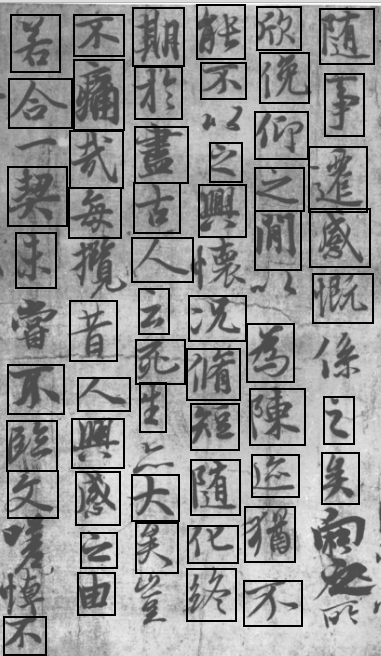
\includegraphics[width=12cm]{cadal-most-characters-boxed.png}}
    \caption{This page has bounding box data for most characters}
    \label{cadal most characters boxed}
    \end{figure}
    
    \begin{figure}{} % page/8938
    \parbox{12cm}{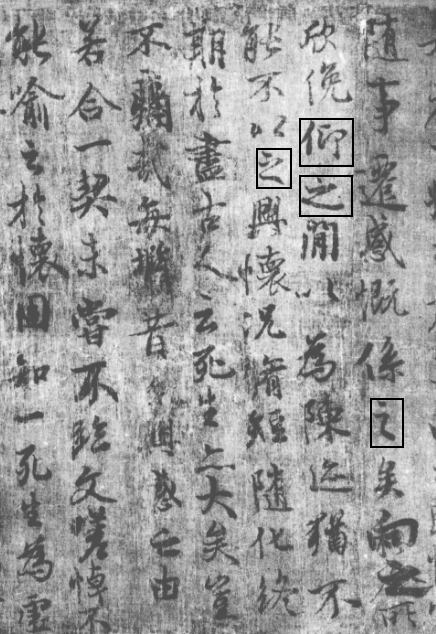
\includegraphics[width=12cm]{cadal-few-characters-boxed.png}}
    \caption{This page has bounding box data for very few characters}
    \label{cadal less characters boxed}
    \end{figure}
    
    \begin{figure}{}
    \parbox{12cm}{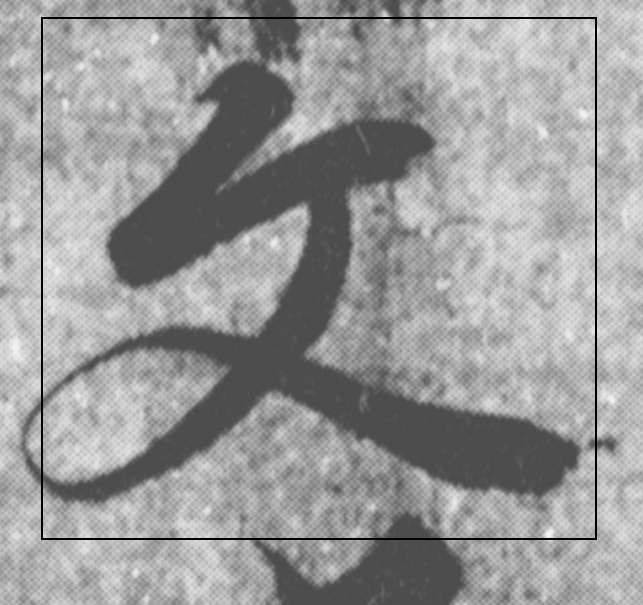
\includegraphics[width=12cm]{cadal-box-missing-part-of-character.png}}
    \caption{Box not covering whole character, and box overlaps a different character when it doesn't have to}
    \label{cadal single character examples}
    \end{figure}
    
    \begin{figure}{}
    \parbox{12cm}{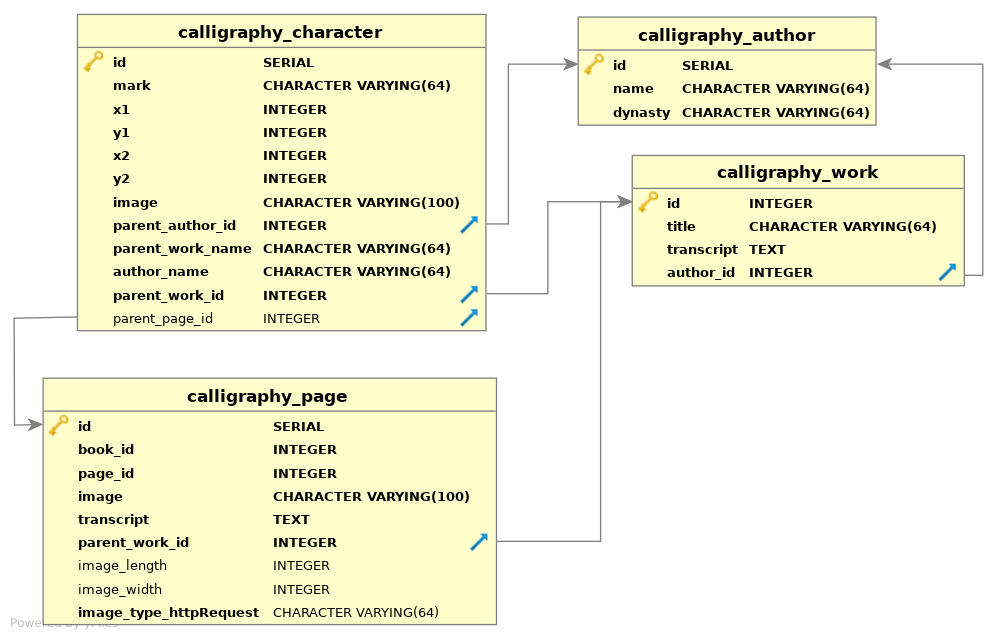
\includegraphics[width=12cm]{calliset-erd.png}}
    \caption{character database in calliset website}
    \label{character database in calliset website}
    \end{figure}
    
